\section{Site graphs}

\subsection{The category of site-graphs}

Define $\kn = \set{A, B,..}$ a set of agent types %with a distinct agent type \emph{free},
and equipped with a site map $\site:\kn\to\nat$.
%such that $\site(\text{free}) = 0$.
Define $\pn$ a set of properties.

%Define the set of external links as follows:
%\[
%\text{Ext} = \set{-,\sfree}\cup\Sigma_{ag}\cup\set{(A,i) : A\in\Sigma_{ag}, i\in\site(A)}
%\]

\begin{definition}[Site-graphs]
A site-graph is a structure $(\ag,\type,\nodes,\links,p_k)$ where
\begin{itemize}
\item $\ag$ is a set of agents, ranged over by $a,b$;
\item $\type:\ag\to \set{A, B,...}$ assigns a type to each agent;
\item $\nodes\subseteq \ag\times\nat\uplus\{\text{free}\}$ is a set of nodes, with a special node free, and where each other node is a pair $(a,i)$ with $a\in\ag$ an agent and $i<\site(\type(a))$ a site of $a$;
\item $\links\subseteq \nodes\times\nodes$ is a set of edges that is \emph{conflict free}: $\forall e,e'\in\links$, $e=e'$ or $e\cap e' \subseteq \{\text{free}\}$;
\item $p_k\subseteq\nodes$, with $k\in\pn$, is the set of internal states of a site. The pairwise intersection of $\{p_k\}_{k\in\pn}$ is the empty set, that is a site can only have one internal state.
\end{itemize}
Denote $\varepsilon$ the empty $\Sigma$-graph.
\end{definition}

%% \begin{property}
%%   A site with a specified property need not be a \emph{specified} site of an agent: $p_k\not\subseteq\sites$.
%% \end{property}
%% Define a partial order on $\links\cup\text{Ext}$:
%% \[
%% - \leq A \leq (A,i) \leq (a,i)
%% \]

\begin{definition}[Morphisms]
A morphism $h:G\to H$ is a total function on agents $h:\ag_G\to\ag_H$ such that
\begin{itemize}
\item it preserves agent's types:
\[
\type(a) = \type(h(a)) \text{ for all }a \in \ag_G
\]
\item it preserves nodes:
\[
\text{ if }(a,i)\in \nodes_G \text{ then }(h(a),i) \in \nodes_H\text{ and }h(\text{free})=\text{free}
\]
\item it preserves property sets:
\[
\set{h(u) : u\in p_{k,G}} \subseteq p_{k,H}, \forall k\in\pn.
\]
\end{itemize}
An embedding or a mono, denoted $h:G\lemb H$, is an injective morphism on edges, that is it preserves edges:
\[
(u,v)\in\nodes_G \implies (h(u),h(v))\in\nodes_H
\]
\end{definition}

\begin{lemma}
  Site-graphs and morphisms form a category.
\end{lemma}

\begin{definition}[Rules]
  \label{def:rule_site}
  A rule is a span $L\overset{h}{\remb} D \overset{g}{\lemb} R$ such that $h$ and $g$ are monos on site graphs and the following hold
  \begin{itemize}
   %\item for any span $L\overset{h'}{\remb} D' \overset{g'}{\lemb} R$ and any embedding $D\overset{f}{\lemb}D'$ such that $h=h'f$ and $g=g'f$ then $f$ is an isomorphism;
  \item $\forall a\in\ag_D$, $(a,i)\in\nodes_D\iff (h(a),i)\in\nodes_L \iff (g(a),i)\in\nodes_R$;
  %\item if $[(g(a),i),x] \in\links_R$ with $x\in\text{Ext}\setminus \sfree$, then $[(h(a),i),x] \in\links_D$;
  %\item if $[(a,i),x] \in\links_R$ and $\nexists b$ such that $h(b)=a$ or $\nexists y$ such that $[(b,i),y]\in\links_D$ then $x\in\sites_R$;
  \item if $a\in\ag_R$ and $a\notin\text{image}(g)$ then $\forall i\in\Sigma_{ag-st}(\type(a))$, $(a,i)\in\nodes_R$ and $\exists e\in \links_R$ such that $(a,i)\in e$.
  \end{itemize}
\end{definition}

\begin{example}
In Kappa, we write rules $L\action R$ and derive the domain of definition. For instance, for the rule
\begin{verbatim}
  A(x!1), C(y!1), B(y) -> A(x!1), C(y), B(y!1)
\end{verbatim}
we obtain the domain of definition \verb|A(x?), C(y?), B(y?)|. This is not in the scope of our paper, please see~\autoref{app:prefix_convention} for more details.
\end{example}

The category of site graphs and morphisms does not have all the pushouts. %but does have all pullbacks.

\begin{example}[Inexistence of pushout in the category of site graphs]
  For the two graphs \verb|A(x!1), B(x!1)| and \verb|A(x)| there is no pushout.
  %% Let $G$, $H$ and $O$ three site graphs defined as follows\footnote{Henceforth we write the symmetric reduction for the set $\links$.}:
  %% \begin{align*}
  %%   \ag_G = \{a\},   \type(a) = A,   \links_G = \{[(a,i),B] \} \\
  %%   \ag_H = \{a'\},  \type(a') = A,  \links_H = \{[(a',i),C]\} \\
  %%   \ag_o = \{a''\}, \type(a'') = A, \links_O = \{[(a'',i),\_]\}.
  %% \end{align*}
  %% There is no site graph $M$ such that the following diagram commutes:
  %% \[
  %% \begin{tikzpicture} %[scale=0.8]
  %%   \node (o) at (0,-1) {\(O\)};
  %%   \node (l1) at (-1.5,0) {\(G\)};
  %%   \node (l2) at (1.5,0) {\(H\)};
  %%   \node (m) at (0,1) {\(M\)};
  %%   \draw [right hook->] (o) -- (l1);
  %%   \draw [left hook->] (o) -- (l2);
  %%   \draw [right hook->] (l1) -- (m);
  %%   \draw [left hook->] (l2) -- (m);
  %% \end{tikzpicture}
  %% \]
\end{example}

\begin{lemma}
  Let $L\overset{h}{\remb} K \overset{g}{\lemb} R$ be a rule and let $M$ and $m:L\emb M$ be a site graph and matching, respectively. The DPO rewriting can be applied whenever the gluing conditions hold.
\end{lemma}
\begin{proof}
  \[
  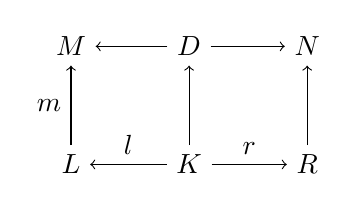
\begin{tikzpicture} %[scale=0.8]
    \node (l) at (-1.5,0) {\(L\)};
    \node (d) at (0,0) {\(K\)};
    \node (r) at (1.5,0) {\(R\)};
    \node (m) at (-1.5,1.5) {\(M\)};
    \node (d') at (0,1.5) {\(D\)};
    \node (n) at (1.5,1.5) {\(N\)};
    \draw [->] (d) -- node [above,midway] {\(l\)} (l);
    \draw [->] (d) -- node [above,midway] {\(r\)} (r);
    \draw [->] (d') -- (m);
    \draw [->] (d') -- (n);
    \draw [->] (l) -- node [left,midway] {\(m\)}  (m);
    \draw [->] (d) -- (d');
    \draw [->] (r) -- (n);
  \end{tikzpicture}
  \]
  Let us first construct $D$ and show that it is the pushout complement. Secondly, we construct $N$ and show that it is the pushout.
  %% \begin{enumerate}
  %% \item

  %% \end{enumerate}
  \begin{mdframed}[backgroundcolor=blue!20]
    to do
  \end{mdframed}
\end{proof}

\begin{mdframed}[backgroundcolor=blue!20]
  \begin{itemize}
  \item stories: posets with an additional relation of non-causal precedence;
\begin{remark}[Stories in Kappa]
In site graph we can express a dependence between events that is neither sequential dependence nor inhibition. It comes from the distinction between low res and medium res influence.

Let us consider an example, with the following three rules

\begin{verbatim}
  r1: C(y),A(x!1,y),B(x!1)-> C(y!2),A(x!1,y!2),B(x!1)
  r2: A(x!1), B(x!1) -> A(x), B(x)
  r3: C(y!2),A(x,y!2) -> C(y!2),A(x~p,y!2)
\end{verbatim}

We have that $r_1\xrightarrow[low]{+} r_3$, $r_2\xrightarrow[medium]{+} r_3$ and $r_2\xrightarrow[medium]{-} r_1$.

Let $e_1$, $e_2$ and $e_3$ be three events such that $r_1$, $r_2$ and $r_3$ are their corresponding labels. We can exhibit contexts for the sequential dependence between $e_2$ and $e_3$ and for the inhibition of $e_1$ by $e_2$, but none of them express the dependence relation between $e_1$ and $e_3$.

Thus, we denote $e<^{\star}e'$ whenever $\labl(e)\xrightarrow[low]{+} \labl(e')$. Stories in Kappa are sets of events equipped with three binary relations $<$, $\dashv$ and $<^{\star}$ and the following properties hold between them:
\begin{align*}
  e < e' \implies e<^{\star}e'\text{ but not the reverse; }\\
\labl(e)\xrightarrow[medium]{+} \labl(e') \implies \labl(e)\xrightarrow[low]{+} \labl(e')\text{ but not the reverse; }\\
  e<^{\star}e'\text{ and }\neg(\labl(e)\xrightarrow[medium]{+} \labl(e'))\implies \exists e'', e''\dashv e\text{ and }e''< e'.
\end{align*}
%% Note that if $e_1\ll e_2$ there are three cases possible:
%% \begin{itemize}
%% \item $e_1< e_2$
%% \item $\labl(e)\xrightarrow{+}\labl(e')$ and $\neg(e_1 < e_2)$
%% \item $\neg(\labl(e)\xrightarrow{+}\labl(e'))$
%% \end{itemize}
\end{remark}

  \item add non-causal precedence to the concretisation function;
  \item no context of inihibition: detect conflict in the site graph.
  \end{itemize}
\end{mdframed}
